% \newpage
\section{Discussion}
\label{sec:discussion}

\subsection{Summarizing results}

This research found that a fine-tuned ResNet50 was able to classify gentrified and non-gentrified signage with an F1-score of 0.69. The model was able to find the same patterns of gentrification in Amsterdam signage characteristics as previous visual qualitative research, in terms of colors and fonts \cite{rahman_signage_2020, trinch_signsays_2017, snajdr_oldschool_2018, snajdr_preserve_2022}, as well as languages \cite{kasanga_map_2012, trinch_signsays_2017}.

Using an image classification model also enabled the study to make conclusions on fuzzy cases, via inspecting the model's misclassified instances. On one hand, there were signs that had the defining characteristics of the opposite class, and thus were identified as such by the model with high certainty. On the other hand, as classification certainty decreased, we were able to see signage with appearances untypical of any class. Variations in fonts and colors were no longer differentiating the classes. Such output showed more nuances in identifying gentrification via signage. Signage alone could not always tell the full story, as signage of non-gentrified facades can still appear gentrified and vice versa, with consistent visual signals found by the model. Especially for the cases of lower classification certainty, the model failed to clearly tell apart gentrified from non-gentrified signs as signals from both classes appeared simultaneously. While we were able to see what signs looked like  beyond the most typical cases of (non-)gentrification (something previous studies did not point out), ultimately, these were the cases that the model failed to distinguish due to added nuances.

Utilizing street view imagery and computer vision also enabled this study to overcome the limitations of past research in terms of generalizability. Past studies, in using labor-intensive manual data collection and qualitative methods, could only make conclusions on a neighborhood scale \cite{reades_understanding_2019, barton_exploration_2016}. Generalizability of the model was tested on a set of extended street view data, label as gentrified and non-gentrified based on census data. Two analyses were done on this set. Firstly, looking at the model's performance, there was a consistent decrease in performance of approximately 10\% in all average metrics. This suggests that given a gentrified neighborhood, not all signage in the neighborhood would be visually perceived as gentrified. Secondly, looking at the model's inference on this data, the same visual patterns were found for both classes. This supports the model's ability to identify the most typical cases of visually (non-)gentrified signs from unseen data on a city-wide scale. An example of detecting gentrification can be seen in Figure \ref{fig:detect_ex}.

% {
% \setlength\intextsep{0pt}
\begin{figure}[h]
    \centering
    \begin{subfigure}[b]{0.22\textwidth}
        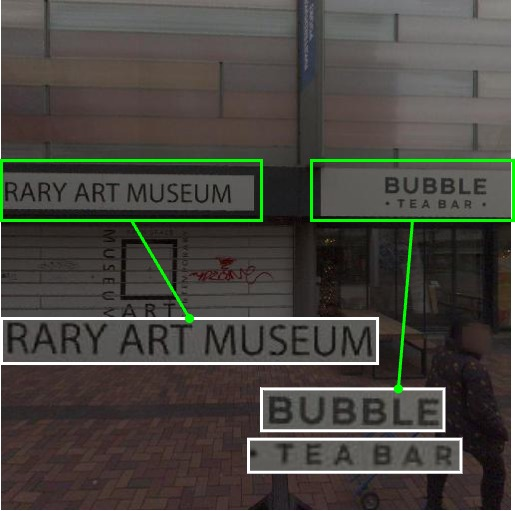
\includegraphics[width=\textwidth]{media/results/detect/detect_ex_gen.jpg}
        \caption{Gentrified: A contemporary art museum \& bubble tea store in the non-gentrified neighborhood of Amsterdamse Poort.}
    \end{subfigure}
    \quad
    \begin{subfigure}[b]{0.22\textwidth}
        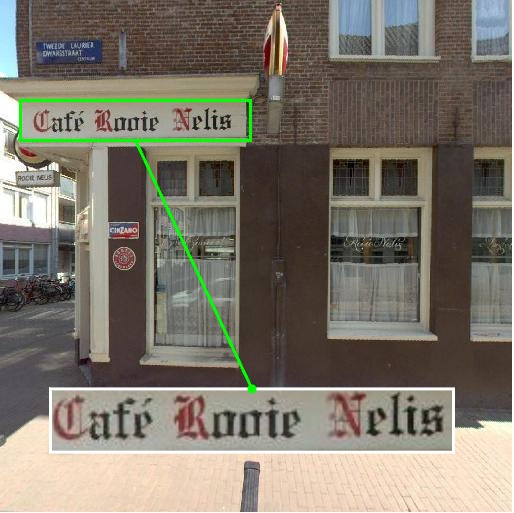
\includegraphics[width=\textwidth]{media/results/detect/detect_ex_non.jpg}
        \caption{Non-gentrified: A classic and reputable Dutch brown cafe in the gentrified neighborhood of De Jordaan.}
    \end{subfigure}
    % \vspace{-2mm}
    \caption{Examples of plausible detection.}
    \label{fig:detect_ex}
\end{figure}
% }

Nonetheless, it is also worth noting that not all detections are reasonable per human perception. Keeping in mind the model's misclassifications on StreetSwipe due to added nuances, we can see some examples of incorrect detection in Figure \ref{fig:detect_inc_ex}. While these are signage of long-established businesses in currently non-gentrified neighborhoods, all but one of them were detected as gentrified.

\begin{figure}[H]
    \centering
    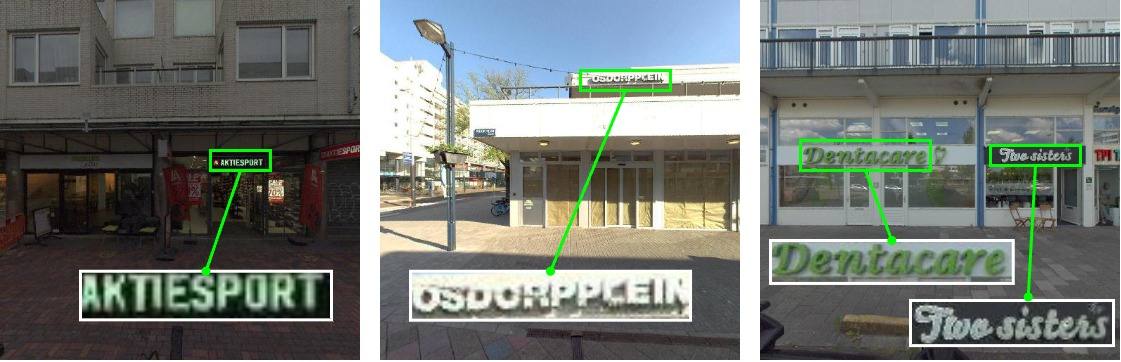
\includegraphics[width=0.5\textwidth]{media/results/detect/detect_inc_ex.jpg}
    \caption{Examples of implausible detection: A sports clothing store in non-gentrified Amsterdamse Poort (left), and a shopping center, dental clinic, and hair salon in non-gentrified Osdorp (middle \& right). With the exception of Dentacare (right), all other signage were classified as gentrified.}
    \label{fig:detect_inc_ex}
\end{figure}

\subsection{Limitations}
\subsubsection{Data-related limitations}

StreetSwipe had the following limitations: 
\begin{itemize}
    \item The number of votes in the pre-july 2020 version of the data was less than in the newer version. This could have lead to lower validity of the results.
    \item There was strong class imbalance, with 75\% of the data belonging to non-gentrified instances. This affected the model's performance in detecting gentrified instances.
    \item The data had varying dates, with some images dating back to 2009. While we technically could still learn perception, as the images were human-annotated in recent years, the results - especially conclusions made about visual characteristics of signage - should not be interpreted as fully representing the most up-to-date state of gentrification in Amsterdam.
\end{itemize}

The extended dataset had a limitation in terms of resolution: Text instances generally had much lower resolutions compared to StreetSwipe, and this is because the street view images were taken from a further distance from facades. This could have contributed to model's lower performance on this set.

\subsubsection{Methodology-related limitations}
The methodology had the following limitations:

\begin{itemize}
    \item Cropping out text instances meant losing information on the entirety of the signage, such as where the text are placed (windows or above the stores' entrances, or standees, posters etc.), text density on signage, text size, total numbers of font types and colors used, which signage type and whether a combination of types (above entrance, on window, standee, neon, backlit) was used. These elements could have served as extra signals for better classification of signage.
    
    \item Cropping out text instances also led to lower reliability for semantic learning. Learning semantic meanings of text could have helped distinguishing between the classes, especially when instances have visual characteristics of the opposite class.

\end{itemize}

\subsection{Future research}
Some avenues for future studies are listed below:
\begin{itemize}
    \item Via object recognition, future studies can include more visual signals by identifying signage in their entirety, and not as (potentially fragmented) text instances. Then, text placement, text density, signage types etc. could be used as features. Further, this would also enable more reliability for semantic learning.

    \item Other features could be combined to aid model accuracy. Other visual indicators include the appearance of the rest of the buildings, what else appeared in the store facade other than signage (e.g. window displays, outdoor seating). Non-visual indicators include types of business, locations, neighborhood socio-economic indicators such as housing prices, residents' age, education level, income, etc. Similar to semantics, these features can further improve classification, especially when signage visual signals are a misdirection for the model.
    
    \item The mismatch in model performance on StreetSwipe and the extended data - or between visual and socio-economic gentrification - points to questions about the neighborhood's demographic makeup. It could be the case that displacement did not happen to old residents, or it did happen but business owners were able to cater to new residents and remained in the gentrified neighborhoods. Indeed, the relationship between gentrification and displacement was found to be more complicated - neighborhood change does not always mean displacement \cite{hochstenbach_anatomy_2015}. A research in this direction calls for combining socio-demographic data in combination with street view imagery. A step further would be to incorporate time series data to enable an analysis into the process of neighborhood change, e.g. whether displacement took place over time, and whether/how aesthetics of the built environment reflected change.
\end{itemize}
